\subsection{Organização do projeto}
Antes de iniciar a implementação, foi definido qual a estrutura de projeto a seguir, pelo que a escolhida foi MVC devido a ser a mais comum e estabelecida. Sendo assim a organização do projeto segue a seguinte estrutura:
\begin{figure}[htb]
  \centering
  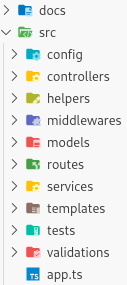
\includegraphics[width=0.2\textwidth]{images/implementacao/api/project_organization.png}
  \caption{Exemplo de página de produto incomum}
  \label{fig:63}
\end{figure}

\begin{itemize}
  \item \textbf{docs} - Documentação gerada;
  \item \textbf{src} - Base de todo o projeto;
  \item \textbf{config} - Ficheiros de configuração do projeto;
  \item \textbf{controllers} - Controladores para cada pedido;
  \item \textbf{helpers} - Ficheiros com funções gerais utilizadas regularmente;
  \item \textbf{middlewares} - Ficheiros com os middlewares da api;
  \item \textbf{models} - Classes criadas para representação de base de dados e para as entidades de resposta;
  \item \textbf{routes} - Rotas existentes;
  \item \textbf{services} - Serviços para cada pedido;
  \item \textbf{templates} - Templates de email a serem enviados;
  \item \textbf{tests} - Testes de código realizados;
  \item \textbf{validations} - Validações a realizar a nível de modelo de negócio e validação de dados;
  \item \textbf{app} - Ficheiro de início do projeto;
\end{itemize}